\documentclass[oneside,a4paper,12pt]{book}
%\usepackage{showframe}
%\hoffset = 8.9436619718309859154929577464789pt
%\voffset = 13.028169014084507042253521126761pt
\usepackage{fancyhdr}

\fancypagestyle{plain}{%
  \fancyhf{}
  \fancyfoot[CE]{Pune Institute of Computer Technology, Department of Computer Engineering 2021 22}
  \fancyfoot[RE]{\thepage}
}
\pagestyle{fancy}
\fancyhead{}
\renewcommand{\headrulewidth}{0pt}
\footskip = 0.625in
\cfoot{}
\rfoot{}

\usepackage[]{hyperref}
\usepackage{tikz}
\usetikzlibrary{arrows,shapes,snakes,automata,backgrounds,petri}
\usepackage{titlesec}
\usepackage{tabularx}

\usepackage[nottoc,notlot,notlof,numbib]{tocbibind}
\usepackage[titletoc]{appendix}
\usepackage{titletoc}
\renewcommand{\appendixname}{Annexure}
\renewcommand{\bibname}{References}

\setcounter{secnumdepth}{5}

\usepackage{float}
\usepackage{subcaption}
\usepackage{multirow}
\usepackage{lmodern}

\begin{document}

\setlength{\parindent}{0mm}
\begin{center}
%{\bfseries SAVITRIBAI PHULE PUNE UNIVERSITY \\}
% \vspace*{1\baselineskip}
{\bfseries A   PROJECT REPORT ON \\}
 \vspace*{2\baselineskip}
{\bfseries \fontsize{16}{15} \selectfont  Medical Image Analysis Using Deep Learning \\ \vspace*{2\baselineskip}}
{\fontsize{12}{12} \selectfont SUBMITTED TO THE SAVITRIBAI PHULE UNIVERSITY, PUNE
 \\ IN THE PARTIAL FULFILLMENT OF THE REQUIREMENTS \\ FOR THE AWARD OF THE DEGREE  \\
 \vspace*{1\baselineskip}
 OF

\vspace*{2\baselineskip}}
{\bfseries \fontsize{14}{12} \selectfont\mbox{BACHELOR OF ENGINEERING (Computer Engineering)} \\
\vspace*{2\baselineskip}} 
{\bfseries \fontsize{12}{12} \selectfont SUBMITTED BY \\ 
\vspace*{2\baselineskip}} 
Mohit Agrawal  \hspace{30 mm}    Exam No:  B150054206 \\
Sarang Mahajan \hspace{28 mm}    Exam No:  B150054364 \\
Urmil Shah     \hspace{37 mm}    Exam No:  B150054437 \\
Rucha Tambe    \hspace{32 mm}    Exam No:  B150054464 \\
\vspace*{2\baselineskip}


\includegraphics[width=100pt]{collegelogo.png} \\
\vskip 0.5cm
{\bfseries \fontsize{16}{15} \selectfont
{\bfseries \fontsize{12}{12} \selectfont 
DEPARTMENT OF COMPUTER ENGINEERING\\
Pune Institute of Computer Technology \\
Dhankawadi, Pune - 411043

\vspace*{1\baselineskip}
SAVITRIBAI PHULE PUNE UNIVERSITY\\
2021-2022
\vspace*{1\baselineskip}
}
\end{center}

\newpage

{\bfseries \fontsize{12}{12} \selectfont }

{\bfseries \fontsize{12}{12} \selectfont }

\begin{figure}[ht]
\centering
\includegraphics[width=100pt]{Pict_logo.png}
\end{figure}

{\bfseries \fontsize{14}{12} \selectfont \centerline{CERTIFICATE} 
\vspace*{2\baselineskip}}

\centerline{This is to certify that the project report entitled}
\vspace*{1\baselineskip} 


{\bfseries \fontsize{12}{12} \selectfont \centerline{ Medical Image Analysis Using Deep Learing}}
{\bfseries \fontsize{12}{12} \selectfont \centerline{  }
\vspace*{1\baselineskip}}

\centerline{Submitted by}
\vspace*{1\baselineskip} 
Mohit Agrawal  \hspace{30 mm}    Exam No:  B150054206 \\
Sarang Mahajan \hspace{28 mm}    Exam No:  B150054364 \\
Urmil Shah     \hspace{37 mm}    Exam No:  B150054437 \\
Rucha Tambe    \hspace{32 mm}    Exam No:  B150054464 \\

\vspace*{1\baselineskip}

is a bonafide student of this institute and the work has been carried out by him/her under the supervision of  \textbf{Prof. D.T.Mane} and it is approved for the partial fulfillment of the requirement of Savitribai Phule Pune University, for the award of the degree of \textbf{Bachelor of Engineering} (Computer Engineering). \\
\\
\vskip 1cm
\bgroup
\def\arraystretch{0.7}
\begin{tabular}{c c }
\textbf{Prof. D.T.Mane} &  \hspace{50 mm} \textbf{Dr. R. B. Ingle} \\
Internal Guide   &  \hspace{50 mm} Head \\
Dept. of Computer Engg.  &	\hspace{50 mm}Dept. of Computer Engg.  \\
\end{tabular}
%}
\begin{center}
%\fontsize{12}{18}\selectfont 
\vspace*{1\baselineskip}
{

\textbf{Dr. P. T. Kulkarni}\\
Principal\\
Pune Institute of Computer Technology  
}
\end{center}
Place:Pune\\
Date:





{  \newpage {\bfseries \fontsize{14}{12} \selectfont \centerline{ACKNOWLEDGEMENT} 
\vspace*{2\baselineskip}} \setlength{\parindent}{11mm} }
{ \setlength{\parindent}{0mm} }
\textit{It gives us great pleasure in presenting the project report 
on {\bfseries \fontsize{12}{12} \selectfont `Medical Image Analysis Using Deep Learning'}.}
\vspace*{1.5\baselineskip}

\justifying{
\noindent
 \textit{We would like to take this opportunity to thank
 \textbf{Prof. D. T. Mane} giving me all the help and guidance we needed. We are
 really grateful to them for their kind support. Their valuable suggestions were very helpful.} 
 }
 \vspace*{1.5\baselineskip}

 \textit{We are also grateful to \textbf{Dr R.B. Ingle}, Head of Computer
 Engineering Department, PICT for his indispensable
 support, suggestions.}
\vspace*{1.5\baselineskip}

\textit{In the end our special thanks to \textbf{Dr. Bhushan Garware}, Persistent Systems Ltd and all faculty members for their whole hearted cooperation for completion of this report. We also thank our laboratory assistants for their valuable help in laboratory.}
\vspace*{3\baselineskip} \\
\begin{tabular}{p{8.2cm}c}
&Mohit Agrawal\\
&Urmil Shah \\
&Sarang Mahajan\\
&Rucha Tambe\\
&(B.E. Computer Engg.)
%}
\end{tabular}

{  \newpage {\bfseries \fontsize{14}{12} \selectfont \centerline{ABSTRACT} 
\vspace*{2\baselineskip}} \setlength{\parindent}{11mm} }
{ \setlength{\parindent}{0mm} }
\textit{Write Abstract here.}
\vspace*{1\baselineskip}

 \vspace*{1.5\baselineskip}

 
\tableofcontents
\listoffigures 




\mainmatter



\titleformat{\chapter}[display]
{\fontsize{16}{15}\filcenter}
{\vspace*{\fill}
 \bfseries\LARGE\MakeUppercase{\chaptertitlename}~\thechapter}
{1pc}
{\bfseries\LARGE\MakeUppercase}
[\thispagestyle{empty}\vspace*{\fill}\newpage]

\setlength{\parindent}{11mm}
\rfoot{Page \thepage}

\pagestyle{fancy}
\fancyhf{}
\lhead{Title of Project}
\cfoot{PICT, Department of Computer Engineering 2021-22}
\rfoot{Page \thepage}
\renewcommand{\headrulewidth}{2pt}
\renewcommand{\footrulewidth}{1pt}

\chapter{Introduction}

\section{Overview}
Overview


\section{Motivation}

\section{Problem Definition and Objectives}

\section{Project Scope \& Limitations }

\section{Methodologies of Problem solving}

\chapter{Literature Survey}




\chapter{Software Requirements Specification}

\section{Assumptions and Dependencies}
In this section, we study the Assumptions and Dependencies of our project, user classes and characteristics along with assumptions and dependencies of our project.

\section{Functional Requirements}
\subsection{System Feature 1(Functional Requirement)}
\subsection{System Feature2 (Functional Requirement)}
\subsection{System Feature n (Functional Requirement)}


\newpage 
\section{External Interface Requirements}


\subsection{User Interfaces}

\subsection{Hardware Interfaces}

\begin{itemize}
    \item 
    \item 
\end{itemize}


\subsection{Software Interfaces}

\begin{enumerate}
\item Operating System: Anyone among MAC OSX, Linux or Windows 
\item Jupyter Notebook
\item Dataset pertinent to medical images
\item Programming Language: Python
\end{enumerate}

\subsection{Communication Interfaces}
\newpage 
\section{Nonfunctional Requirements}
    \subsection{Performance Requirements}
    \subsection{Safety Requirements}
    \subsection{Security Requirements}

    \subsection{Software Quality Attributes}
  


\section{System Requirements}
\subsection{Database Requirements}
\subsection{Software Requirements (Platform Choice)}
\subsection{Hardware Requirements}

\section{Analysis Models: SDLC Model to be applied}



\newpage


\chapter{System Design}

\section{System Architecture}



\section{Mathematical Model}
Mathematical Model

\section{Data Flow Diagrams}

A description of each major software function, along with data flow (structured analysis) or class hierarchy (Analysis Class diagram with class description for object oriented system) is presented. 

\begin{center}
	\begin{figure}[!htbp]
		\centering
		\fbox{\includegraphics[width=300pt]{DFD0.jpg}}
	  \caption{Data Flow Diagram}
	  \label{fig:usecase}
	\end{figure}
\end{center}


\begin{center}
	\begin{figure}[!htbp]
		\centering
		\fbox{\includegraphics[width=300pt]{DFD1.jpg}}
	  \caption{Data Flow Diagram}
	  \label{fig:usecase}
	\end{figure}
\end{center}

\begin{center}
	\begin{figure}[!htbp]
		\centering
		\fbox{\includegraphics[width=300pt]{DFD2.jpg}}
	  \caption{Data Flow Diagram}
	  \label{fig:usecase}
	\end{figure}
\end{center}


\section{Entity Relationship Diagram}

Here, we have shown how two different entities will interact using the system architecture.
\begin{center}
	\begin{figure}[!htbp]
		\centering
		\fbox{\includegraphics[width=\textwidth]{usecase.jpg}}
	  \caption{Use case diagram}
	  \label{fig:usecase}
	\end{figure}
\end{center}

\\    
\section{UML Diagrams}

\begin{center}
	\begin{figure}[!htbp]
		\centering
		\fbox{\includegraphics[width=300pt]{activity.png}}
	  \caption{Activity Diagram}
	  \label{fig:usecase}
	\end{figure}
\end{center}

\newpage


\newpage

\section{Sequence Diagram}
 \begin{center}
	\begin{figure}[!htbp]
		\centering
		\fbox{\includegraphics[width=450pt]{sequence.png}}
	  \caption{Sequence Diagram}
	  \label{fig:class dig}
	\end{figure}
\end{center}

\chapter{Project Plan}

\section{Project Estimate}
\subsection{Reconciled Estimates}

\begin{itemize}
    \item Reconciled Estimates
    \item Reconciled Estimates
    \item Reconciled Estimates
    \item Reconciled Estimates
    
\end{itemize}
\subsection{Project Resources}

\newpage
\section{Risk Management}
\begin{itemize}
\item Risk Management
\end{itemize}

\subsection{Risk Identification}
\begin{itemize}
\item Risk Identification
\end{itemize}
\subsection{Risk Analysis}
\begin{itemize}
    \item Risk Analysis
\end{itemize}
\subsection{Overview of Risk Mitigation, Monitoring, Management}
\begin{itemize}
    \item Overview of Risk Mitigation, Monitoring, Management
\end{itemize}

\newpage
\section{Project Schedule}

\subsection{Project Task Set}
\begin{itemize}
    \item Project Task Set
\end{itemize}

\subsection{Task Network}
\begin{itemize}
    \item Task Network
\end{itemize}

\subsection{Timeline Chart}
\caption{Timeline Chart}
\begin{itemize}
    \item Timeline Chart
\end{itemize}

\section{Team Organization}

\subsection{Team structure}
\begin{itemize}
    \item Team structure
\end{itemize}

\subsection{Management reporting and communication}
\begin{itemize}
    \item Management reporting and communication
\end{itemize}


\chapter{Project Implementation}
 
\section{Overview of Project Modules}
\begin{itemize}
    \item Overview of Project Modules
\end{itemize}



\section{Tools and Technologies Used}
\begin{itemize}
    \item Tools and Technologies Used
\end{itemize}


\section{Algorithm Details}
\subsection{Algorithm 1}
\subsection{Algorithm 2}
\subsection{Algorithm 3}

\todo{Add as many Algorithm subsections}

\newpage
\chapter{Software Testing}

\section{Type of Testing}
\begin{itemize}
    \item Type of Testing
\end{itemize}

\section{Test cases \& Test Results}
\begin{itemize}
    \item Test cases \& Test Results
\end{itemize}

\chapter{Results}

\section{Outcomes}
\begin{enumerate}
    \item Outcome 1
\end{enumerate}

\begin{enumerate}
    \item Outcome 2
\end{enumerate}

\begin{enumerate}
    \item Outcome 3
\end{enumerate}

\section{Screen Shots}
 \begin{center}
	\begin{figure}[!htbp]
		\centering
		\fbox{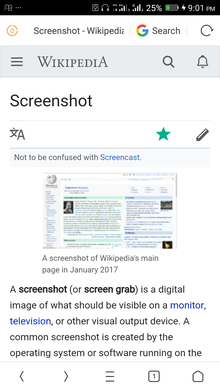
\includegraphics[width=300pt]{screenshot.png}}
	  \caption{Screenshot}
	  \label{fig:screenshot}
	\end{figure}
\end{center}

\newpage
\chapter{Conclusions}

\section{Conclusions}
\begin{enumerate}
    \item Conclusion 1
\end{enumerate}

\section{Conclusions}
\begin{enumerate}
    \item Conclusion 2
\end{enumerate} 

\section{Conclusions}
\begin{enumerate}
    \item Conclusion 3
\end{enumerate}

\section{Future Work}
\begin{enumerate}
    \item Future Work
\end{enumerate}

\section{Applications}
\begin{enumerate}
    \item Applications
\end{enumerate}
    

\chapter{Appendix}

\section{Appendix A}

\todo{Problem statement feasibility assessment using, satisfiability analysis and NP Hard, NP-Complete or P type using modern algebra and relevant mathematical models.}





\newpage
\section{Appendix B}

\todo{Details of paper publication: name of the conference/journal, comments of reviewers, certificate, paper.}


\newpage
\section{Appendix C}

\todo{Plagiarism Report of project report.}


\begin{thebibliography}{99}

\bibitem{c1}

\bibitem{c2}
\bibitem{c3}

\bibitem{c4} 
\bibitem{c5}

\bibitem{c6}

\bibitem{c7}

\bibitem{c8}

\bibitem{c9}
\bibitem{c10}

\bibitem{c11}

\end{thebibliography}




\newpage

\begin{table}[]
\centering
\renewcommand{\arraystretch}{1.5}


\caption*{LIST OF ABBREVATIONS}
\begin{tabular}{|l|l|}
\hline
Abbreviation & Illustration                                                               \\ \hline

VPN          & \begin{tabular}[c]{@{}l@{}}Virtual\\ 			Private Network\end{tabular}       \\ \hline
IP           & \begin{tabular}[c]{@{}l@{}}Internet\\ 			Protocol\end{tabular}             \\ \hline
IDS          & \begin{tabular}[c]{@{}l@{}}Intrusion\\ 			Detection System\end{tabular}    \\ \hline
TCP          & \begin{tabular}[c]{@{}l@{}}Transmission\\ 			Control Protocol\end{tabular} \\ \hline
\end{tabular}
\end{table}




\pagebreak
\newpage


\begin{table}[]
\centering
\caption*{LIST OF FIGURES}
\renewcommand{\arraystretch}{1.3}
\begin{tabular}{|l|l|l|}
\hline
Figure & Illustration                                                   & Page No. \\ \hline

1.1    & \begin{tabular}[c]{@{}l@{}}System\\ 			Overview\end{tabular}   & 3        \\ \hline
1.2    & \begin{tabular}[c]{@{}l@{}}System\\ 			Behavior\end{tabular}   & 5        \\ \hline
2.1    & \begin{tabular}[c]{@{}l@{}}TCP\\ 			Header\end{tabular}        & 11       \\ \hline
4.1    & \begin{tabular}[c]{@{}l@{}}Waterfall\\ 			Model\end{tabular}   & 27       \\ \hline
4.2    & \begin{tabular}[c]{@{}l@{}}Timeline\\ 			Chart\end{tabular}    & 30       \\ \hline
4.3    & \begin{tabular}[c]{@{}l@{}}DFD\\ 			Level 0\end{tabular}     & 31       \\ \hline
4.4    & \begin{tabular}[c]{@{}l@{}}DFD\\ 			Level 1\end{tabular}     & 32       \\ \hline
4.5    & \begin{tabular}[c]{@{}l@{}}DFD\\ 			Level 2\end{tabular}     & 33       \\ \hline
4.6    & \begin{tabular}[c]{@{}l@{}}Use\\ 			case Diagram\end{tabular}  & 34       \\ \hline
4.7    & \begin{tabular}[c]{@{}l@{}}Sequence\\ 			Diagram\end{tabular}  & 35       \\ \hline
4.8    & \begin{tabular}[c]{@{}l@{}}ER\\ 			Diagram\end{tabular}        & 36       \\ \hline
4.9    & \begin{tabular}[c]{@{}l@{}}Class\\ 			Diagram\end{tabular}     & 37       \\ \hline
4.10   & \begin{tabular}[c]{@{}l@{}}Component\\ 			Diagram\end{tabular} & 38       \\ \hline
4.11   & \begin{tabular}[c]{@{}l@{}}Deployment\\ 			Diagram\end{tabular} & 39       \\ \hline
4.12   & \begin{tabular}[c]{@{}l@{}}State Machine\\ 			Diagram\end{tabular} & 40       \\ \hline
\end{tabular}
\end{table}

\pagebreak

\newpage

\begin{table}[]
\centering
\renewcommand{\arraystretch}{1.5}
\caption*{LIST OF TABLES}

\begin{tabular}{|l|l|l|}
\hline
Table & Illustration                                                    & Page No. \\ \hline

4.1   & \begin{tabular}[c]{@{}l@{}}Project\\ 			Plan\end{tabular}       & 29       \\ \hline
3.1   & \begin{tabular}[c]{@{}l@{}}Packet\\ 			Information\end{tabular} & 47       \\ \hline
3.2   & \begin{tabular}[c]{@{}l@{}}Network\\ 			Error\end{tabular}      & 48       \\ \hline
3.3   & \begin{tabular}[c]{@{}l@{}}IP\\ 			Configuration\end{tabular}   & 48       \\ \hline


\end{tabular}
\end{table}

\end{document}